\documentclass[a4paper,12pt]{article}
%\usepackage{t1enc}
\usepackage[longnamesfirst, round]{natbib}  % Bindet den natbib-standard fuer das Zitieren ein
%\usepackage{epsfig}
\usepackage[latin1]{inputenc}   % Ermoeglicht Sonderzeichen direkt einzugeben
\usepackage[T1]{fontenc}        % Garantiert saubere Worttrennung bei Umlauten etc.
\usepackage{color}              % Farbpaket
\usepackage[fleqn]{amsmath}
\usepackage{amsfonts,amssymb}   % ermoeglicht mathematische Sonderzeichen
%\usepackage{ngerman}           % neue deutsche Rechtschreibung
\usepackage[english]{babel}     %
\usepackage{ae}                 %
\usepackage{graphicx}           % Ermoeglicht das Einbinden von Bildern in allen Formaten
\usepackage{longtable}          % zum erstellen von Tabellen ber mehrere Seiten
\usepackage{multirow}           % zum Verbinden von Zeilen innerhalb einer Tabelle
\usepackage{pictexwd}           % PicTex, ein Graphikpaket
\usepackage{pst-all, multido}   % psTricks, ein Graphikpaket
\usepackage{url}
\usepackage[font=small,labelfont=bf]{caption}
\usepackage{amsmath} %for hats 
\usepackage{dcolumn}
\usepackage{amsthm}
\usepackage[font={footnotesize}]{caption}
\captionsetup[figure]{justification=raggedright,singlelinecheck=false}
\usepackage[super]{nth} %only for 1st 2nd 3rd etc
\usepackage{appendix}
\usepackage{dcolumn}
\usepackage{pdflscape}
\usepackage{booktabs}
\usepackage{threeparttable}
\usepackage{rotating}
\usepackage{hyperref}

% ________________ EINRICHTEN DES DOKUMENTS ______________________%

\bibliographystyle{plainnat}    % legt den Stil fuer das Inhaltsverzeichnis fest

\oddsidemargin 0.0in \evensidemargin 0.0in \textwidth 15.5cm \topmargin -0.4in \textheight 24.5cm \hoffset 0.31in
\parindent 0.7cm      % legt die Seitenraender fest

\pagestyle{plain}          % leere Kopfzeile, Seitennummer in der Mitte der Fusszeile

%\newcommand{\bs}{\boldsymbol}  % shortcut zur Erzeugung von fetten Sympolen in der Mathe-Umgebung

\renewcommand{\baselinestretch}{1.25}
% 1,5 -facher Zeilenabstand (Standard ist 1,2-facher Zeilenabstand, also 1,2*1,25 = 1,5

\usepackage{array, boldline, makecell, booktabs}

%\newcommand\btrule[1]{\specialrule{#1}{0pt}{0pt}}
%\usepackage[svgnames, table]{xcolor}

\begin{document}

% ________________ TITELSEITE ______________________%


\pagenumbering{roman}   % roemische Zahlen zur Seitennumerierung

\begin{titlepage}       % Umgebung fuer Titelseite, frei gestaltbar

\thispagestyle{empty}   % keine Numerierung auf Titelseite


\begin{center}
\vspace*{2.5cm}
{\bf  \Large   Economic Cost of Crime }\\
\vspace*{3cm} 
Term Paper\\
Prof. Dr. Nora Markwalder and Dr. Monika Simmler
\\ Criminology Class\\

\vspace*{0.5cm} 
December \nth{20}, 2020\\
\end{center}

\vfill
\begin{flushright}
   \emph{Erik-Jan Senn} \\
    \emph{Langgasse 56}\\
    \emph{9008 St. Gallen}\\

\end{flushright}



% 
% \begin{center}
% $ $			% oeffnet und schliesst eine Matheumgebung (Trick, um den Titel nach unten zu rutschen
% \vspace{4cm}
% 
% {\LARGE TITEL}
% \vskip 4cm
% 
% Diese Seite ist frei gestaltbar
% \end{center}

\end{titlepage}

\newpage                % erzwingt an dieser Stelle einen Seitenumbruch


% ________________ Antiplagiatserklärung ______________________%


% ________________ INHALTSVERZEICHNIS ______________________%

\newpage
\tableofcontents   %fuegt Automatisch ein Inhaltsverzeichnis ein

\listoftables 

\listoffigures
% 
\newpage
% 


% ________________ HAUPTTEIL ______________________%



\pagenumbering{arabic}      % Seitenzahlen wieder arabisch numerieren
\setcounter{page}{1}        % Ruecksetzen des Seitenzahlzaehlers auf 1


\subsection*{\textit{Abstract}}

\textit{Abstract}


\section{Introduction}
\label{Introduction}
Economic cost of crime are any cost associated with the prevention or the consequences of criminal activities and is usually measured in monetary units.
This general definition can refined in tangible and intangible economic cost of crime.
Tangible costs are measured in a monetary value already which makes them easy to estimate. They include direct cost such as repair cost for damaged goods, cost for medical care, cost for police and justice services and indirect cost such as prevention cost, loss of economic output (goods, services) or lost tax revenue.
Intangible costs need to be transformed into a monetary value and are harder to measure. Examples are experienced pain, reduces quality of live of victims, fear of persecution of the offender or reduces trust in strangers for the entire society (see Table \ref{fig:unit_cost_crime}). \citep{kosten_nutzen_entorf} 

The first crime cost estimation method discussed in this paper tries to estimate each component of cost separately and then sums up the components.
This "detailed" estimation of crime cost could be used to evaluate justice policy using cost and benefit analysis. Take this simple question as an example: Is it profitable to introduce police patrols in cities at night? The question could be answered from an economic perspective if estimates for the following aspects are available: (1) cost for police patrols, (2) changes in prevented, detected and committed crimes due to police patrols and (3) economic cost of crime for each individual crime that is affected by police patrols. If that is the case, we could evaluate the question by comparing the cost of the measure (1) and the benefits of the measure (combine (2) and (3)).
However, apart from (1) which mainly consists of direct cost, it is hard to find sufficient data for estimate (2) and (3). Unit crime costing methods as described in Section \ref{Literature Review} estimate the cost of an individual crime as required for (3), but results show a high variation in cost and are mainly available for the US. 
Overall, the idea of using cost and benefit analysis for justice policy evaluation is often not feasible because especially intangible cost of crime are hard to measure.

The second crime cost estimation method does not attempt to capture each cost component separately (e.g. does not differentiate between tangible and intangible cost) and calculate a static cost estimate - it tries to estimate an effect of criminal activity on economic outcomes.
Specifically, the short empirical analyses of this paper is based on the idea of \citep{entorf} and tests if crime rates negatively impact GDP-growth of countries in Europe. 
Compared to the question-specific and case specific analysis first method, this approach requires less data and could potentially capture more unobserved effects such as a change in victims risk tolerance or reduced trust in society due to crime.
Because economic outcome variables are also impacted by non-crime related factors, additional control variables need to be introduced and the effect measure is more noisy. 
Also, this more general analysis reduces the usability of the analysis for policy evaluation because many macro-variables cannot be directly influenced by an institution.\footnote{Justice system characteristics that are easier to impact such the share of prisoners or police expenditure would give a more direct interpretation and enhance the relevance of the analysis.} While static quantified effects in terms of overall economic variables are hard to interpret, the impact if crime on the dynamics of economic variables could be easier to grasp. \footnote{For example, it might be more interesting that criminal activity reduces the GDP by 0.5\% this year than to know that criminal activity accounts for 3 \% of the GDP.} 

The paper is organized as follows: Section \ref{Literature Review} gives an overview of the existing literature for crime-costing methods and more broad analysis approaches such as in this paper. Section \ref{Methodology} introduces the empirical method, Section \ref{Data} the data used. Section \ref{Results} presents the empirical results and Section \ref{Conclusion} concludes. 

\begin{figure}
\begin{minipage}{0.9\textwidth}
  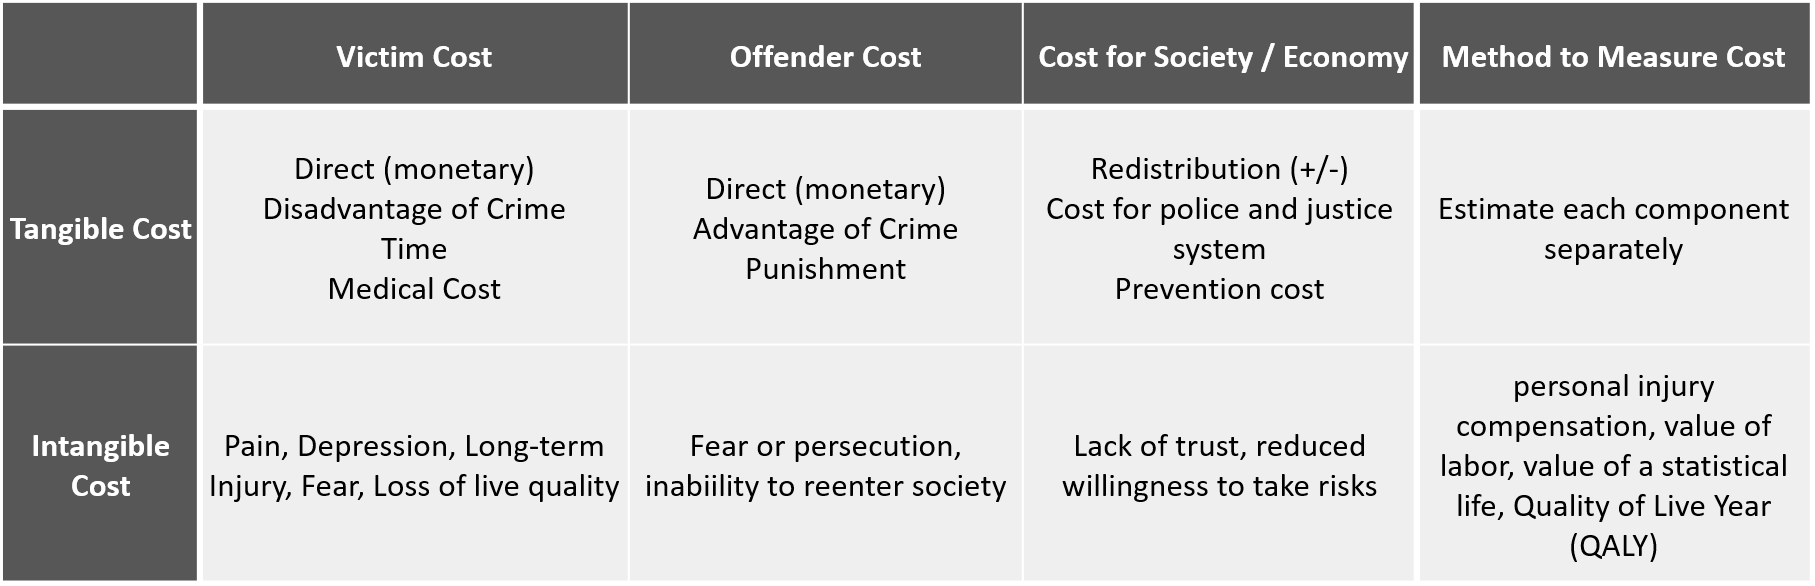
\includegraphics[trim={0 0 0 0},width=\linewidth]{charts/table_unit_cost.png}
\begin{flushleft}
\captionof{figure}{Cost of Crime - Classification}
\footnotesize{\textit{Note:} The table shows examples of cost of crime components classified in different categories and potential ways to measure the components separately. Source: own representation.
\label{fig:unit_cost_crime}	
}
\end{flushleft}
\end{minipage}
\end{figure}


\section{Literature review}
\label{Literature Review}
The literature can be broadly divided into the two estimation methods discussed: the data-reliant detailed crime-costing methods that calculate cost of individual components and the less data-reliant macro perspective approaches. 


\subsection{Unit Crime Costing}
First, for crime-costing methods, most research that includes intangible cost has been conducted in the US due to the availability of tangible cost data. 
For intangible cost, various different approaches are used. 
The idea of a statistical value of a life (SVL) assigns a monetary value to a life e.g. by discounting the expected economic value generated by one person to the current date. It can be interpreted as the economic loss of death. \cite{viscusi} estimates the SVL to be 2 million USD at that time, more current estimates are generally higher due to inflation.
The "jury compensation approach" by \citep{cohen1988} uses the SVL and historical risk of death for different crime categories to estimate intangible unit crime cost. However, this approach does not take other consequences such as disabilities or psychological issues into account.
Cost-of-illness approaches distinguish between different types of injuries. For example, determined monetary payments for injuries from health insurance or personal injury compensation payments determined by court could be used to value economic cost for the victim more accurately. 
The Quality-Adjusted-Life-Year (QALY) measure from health economics is a numeric indicator between 0 and 1 that makes different health issues comparable. The willingness-to-pay to prevent a reduction in QALY can be estimated using surveys \citep{entorf}.
Similarly, the willingness-to-pay approach of \citep{cohen2004} values a crime by asking how much someone is willing to pay to reduce the chance of being a victim. \footnote{For example, if someone is willing to pay 100 USD to reduce the change of robbery by 10 \% , the estimated cost per case is 1,000 USD.} 
While all of these approaches mentioned might include most considerations of potential victims and offenders regarding a crime, they might not fully reflect intangible cost society such as mistrust or reduces willingness to take risks.

\cite{collister} show a summary of unit-cost of crime study results with different methods (see Table \ref{fig:unit_cost_crime_lit_review}). 
The type of offense has a large impact on the cost of crime estimates: estimates for violent crimes are higher than for property crimes, mostly due to medical cost, justice system cost and intangible cost. Murder has the highest estimated cost for every study, which can be explained by the economic loss of a life and high tangible cost of a murder. 
Also, the unit cost estimates show strong variation across studies - the cost of robbery estimate for example lies between 18,591 USD and 280,237 USD. 

It is possible to use unit cost estimates to estimate the aggregated cost of crime by combining it with the case numbers. However, economically it could more plausible to see the cost estimates as marginal cost because cost per case might change with more or less cases due to economies of scale for the justice system or a potential critical threshold of crime that could lead to an economic breakdown. Common estimates of 3\% to 7\% of GDP for developed countries as in \citep{kosten_nutzen_entorf} could be seen with some caution. 

\begin{figure}
\begin{minipage}{0.9\textwidth}
  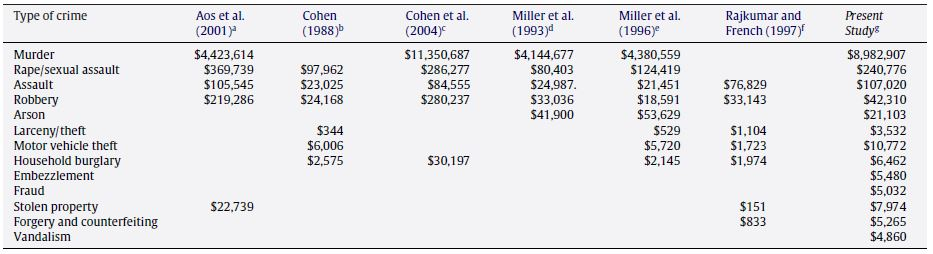
\includegraphics[trim={0 0 0 0},width=\linewidth]{charts/tab_lit_review.jpg}
\begin{flushleft}
\captionof{figure}{Unit Cost of Crime}
\footnotesize{\textit{Note:} This table from \cite{collister} shows a summary of unit cost of crime estimates in the literature for different types of crimes. Source: \cite{collister}.
\label{fig:unit_cost_crime_lit_review}	
}
\end{flushleft}
\end{minipage}
\end{figure}

\subsection{Macro Perspective}
The second approach discussed in this paper does not estimate a static cost of crime based on separate cost estimations, but interprets "cost" more broadly as the effect of crime on economic measures. Researchers use times series data of socio-economic indicators and crime measures of multiple regions. All papers presented here use a more or less sophisticated version of an auto-regressive (AR) model: the basic idea of an AR model is that past observations of the dependent help to explain future ones. 

Each effect estimation in this section consists of, firstly, an economic outcome variable such as GDP-growth or unemployment as dependent variable, secondly, one or multiple measures of crime such as case data for categories of crime or a crime index and, thirdly, a set of control variables that explains variation in economic outcomes that do are not connected with crime. 

The main model for the empirical section of this paper stems from \cite{entorf} and uses a simple AR(1) model for GDP-growth controlling only for investment. They use data for EU-countries from Eurostat - the same database that is also used for this analysis (but here with more current data). 
In Section \ref{Methodology}, this sparse model will be adapted to control for more variables and a different crime measure will be introduced.
\cite{detotto} use the same idea with a more flexible model specification allowing for more long run effects using Italian crime data.

\cite{var_model} use a even more flexible vector-auto-regressive model to model the relationship between homicide rate shocks and the economic variables GDP-growth and foreign direct investment. In a VAR-model as the general case of an AR-model, not only one, but multiple dependent variables are explained simultaneously and can impact each other. Their analysis using data from 32 Mexican states accounts for reverse causality (GDP-growth affects crime) and unknown time delay of effects and finds a GDP-growth reduction of 0.25\% after a shock of homicide rates.

\cite{columbia} investigate whether crime in Columbia had a significant effect on economic growth. In a similar way to the studies above, they use a cross section of economic indicators including education for all countries worldwide to explain log GDP per capita. They tackle reverse causality issues using instrumental variables for human capital and institutional power. However, they do not directly observe a crime measure, but simply include a dummy for Columbia and claim this is a measure of criminal activity. This seems like a strongly simplified approach because this dummy can also include other systematic differences in economic dynamics. 



\section{Methodology}
\label{Methodology}
Goal: not a model for gdp, but try to see if variation in gdp can have anything to do  (modeling gdp is generally hard

What to use as y-variable?
BIP: problem - excludes illegal activity by definition.

Which crime measures?
all crime rates separately, then test jointly
PCA index idea - just see what happens


Causal Model Idea
Causal: 4 assumptions. 
Panel Data Fixed effects.
Confounder description: 

Potential issues: 
missing confoudners - factors that differ in eu countries are not explained by confounders and not constant over time
high variance of model (gdp hard to explain)
reverse causality
no sufficient heterogeneity in crime rates accross europe

\section{Data}
\label{Data}
\subsection{Source}
Aim: estimate for european countries

IN SWITZERLAND: 

For example, in Switzerland the cost for only the penal system can only 1 bill (also a request

0.22\% of GDP (gross domestic product) is spend on the court system
In 2014 a request from the Christian Democratic Party (CVP) to the Swiss parliament asked to investigate the economic cost of crime in order to make more efficient investments in prevention and the justice system. The request was turned down due to the high cost to conduct the analysis.\citep{postulat}.

IN EU: no detailed data anymore (only country level)

Requirements for data, weaknesses

did not remove financial crisis because only 10 years

\subsection{Descriptives}
GDP, 
scatter PCA
pca loadings \& crime index to veryfiy crime index constructzion
should be checked more with existing crime measures
pca factor loadings: interestingly, homicide negative, others pos -> homicide weird, but kept as it is (point to discuss). CHANGE SIGN FOR PCS
BUT: purpose of crime measure is NOT to compare across countries, but to compare years within the same country -> therefore a consistent construction of the measure is enough

number obs 269, 10 years
% latex table generated in R 3.6.1 by xtable 1.8-4 package
% Sat Dec 19 22:03:14 2020
SUMMARY STATS
\begin{table}[ht]
\centering
\begin{tabular}{rrrrrr}
  \hline
 & Mean & Median & St.-Dev. & Mean - Low Crime & Mean - High Crime \\ 
  \hline
pc\_crime\_1 & -0.03 & -0.43 & 1.74 & -0.22 & 0.18 \\ 
  pc\_crime\_2 & -0.01 & -0.21 & 1.19 & -0.06 & 0.05 \\ 
  binary\_crime & 0.43 & 0.00 & 0.50 & 0.43 & 0.43 \\ 
  binary\_crime\_country & 0.47 & 0.00 & 0.50 & 0.00 & 1.00 \\ 
  gdp & 1.54 & 1.90 & 3.37 & 2.20 & 0.80 \\ 
  gdp\_lag1 & 1.41 & 1.80 & 3.39 & 2.00 & 0.74 \\ 
  inflation\_lag1 & 97.03 & 99.10 & 5.16 & 97.64 & 96.34 \\ 
  investment\_lag1 & 21.23 & 21.21 & 3.72 & 20.87 & 21.62 \\ 
  poverty\_lag1 & 24.68 & 21.20 & 8.66 & 24.61 & 24.76 \\ 
  educ\_university & 38.53 & 40.70 & 9.99 & 39.80 & 37.12 \\ 
  educ\_secondary & 77.53 & 80.70 & 13.12 & 78.87 & 76.03 \\ 
  young\_males & 17.44 & 17.40 & 1.09 & 17.24 & 17.66 \\ 
   \hline
\end{tabular}
\end{table}

% latex table generated in R 3.6.1 by xtable 1.8-4 package
% Sat Dec 19 21:51:11 2020
FACTOR LOADINGS
\begin{table}[ht]
\centering
\begin{tabular}{rrrrrrrr}
  \hline
 & Comp.1 & Comp.2 & Comp.3 & Comp.4 & Comp.5 & Comp.6 & Comp.7 \\ 
  \hline
intentional\_homicide\_1 & -0.23 & 0.22 & 0.84 & 0.41 & 0.05 & 0.07 & 0.12 \\ 
  assault\_2 & 0.27 & 0.60 & 0.10 & -0.23 & -0.66 & -0.23 & -0.11 \\ 
  sexual\_violence\_3 & 0.46 & -0.08 & 0.29 & -0.31 & 0.43 & -0.59 & 0.28 \\ 
  robbery\_4 & 0.27 & 0.63 & -0.11 & -0.09 & 0.52 & 0.49 & -0.02 \\ 
  burglary\_5 & 0.47 & -0.04 & -0.22 & 0.55 & -0.21 & 0.10 & 0.61 \\ 
  theft\_5 & 0.50 & -0.15 & 0.07 & 0.44 & 0.07 & -0.08 & -0.72 \\ 
  drugs\_6 & 0.35 & -0.41 & 0.37 & -0.42 & -0.23 & 0.58 & 0.03 \\ 
   \hline
\end{tabular}
\end{table}



\section{Results}
\label{Results}
Issue of method: need long time dimension, cross section only helps to estimate effects of other coefficeints. Cross-sectional variation does not matter here (but if I use the other measure, get a clearly negative effect -> however, this is wrong!

\singlespacing{
\begin{table}[!htbp] \centering 
  \caption{HI} 
  \label{} 
\begin{tabular}{@{\extracolsep{5pt}}lcccc} 
\\[-1.8ex]\hline 
\hline \\[-1.8ex] 
 & \multicolumn{4}{c}{\textit{Dependent variable:}} \\ 
\cline{2-5} 
\\[-1.8ex] & \multicolumn{4}{c}{gdp} \\ 
\\[-1.8ex] & (1) & (2) & (3) & (4)\\ 
\hline \\[-1.8ex] 
 pc\_crime\_1 & 0.594 &  &  &  \\ 
  & (0.445) &  &  &  \\ 
  & & & & \\ 
 pc\_crime\_2 &  & 0.653 &  &  \\ 
  &  & (0.636) &  &  \\ 
  & & & & \\ 
 binary\_crime &  &  & $-$0.801 &  \\ 
  &  &  & (1.010) &  \\ 
  & & & & \\ 
 binary\_crime\_country &  &  &  & 0.022 \\ 
  &  &  &  & (0.331) \\ 
  & & & & \\ 
 gdp\_lag1 & 0.152$^{**}$ & 0.158$^{**}$ & 0.160$^{**}$ & 0.158$^{**}$ \\ 
  & (0.063) & (0.063) & (0.064) & (0.064) \\ 
  & & & & \\ 
 inflation\_lag1 & $-$0.048 & $-$0.027 & $-$0.041 & $-$0.041 \\ 
  & (0.054) & (0.055) & (0.054) & (0.055) \\ 
  & & & & \\ 
 investment\_lag1 & $-$0.089 & $-$0.098 & $-$0.095 & $-$0.097 \\ 
  & (0.064) & (0.064) & (0.064) & (0.064) \\ 
  & & & & \\ 
 poverty\_lag1 & 0.088 & 0.075 & 0.084 & 0.080 \\ 
  & (0.096) & (0.096) & (0.096) & (0.096) \\ 
  & & & & \\ 
 educ\_university & 0.025 & 0.009 & 0.014 & 0.017 \\ 
  & (0.065) & (0.066) & (0.065) & (0.065) \\ 
  & & & & \\ 
 educ\_secondary & 0.118 & 0.123 & 0.109 & 0.119 \\ 
  & (0.077) & (0.077) & (0.078) & (0.077) \\ 
  & & & & \\ 
 young\_males & 0.147 & 0.058 & 0.270 & 0.206 \\ 
  & (0.364) & (0.390) & (0.370) & (0.363) \\ 
  & & & & \\ 
\hline \\[-1.8ex] 
Observations & 269 & 269 & 269 & 269 \\ 
R$^{2}$ & 0.657 & 0.656 & 0.655 & 0.654 \\ 
Adjusted R$^{2}$ & 0.582 & 0.581 & 0.580 & 0.579 \\ 
Residual Std. Error (df = 220) & 2.181 & 2.184 & 2.186 & 2.189 \\ 
F Statistic (df = 48; 220) & 8.774$^{***}$ & 8.730$^{***}$ & 8.704$^{***}$ & 8.667$^{***}$ \\ 
\hline 
\hline \\[-1.8ex] 
\textit{Note:}  & \multicolumn{4}{l}{$^{*}$p$<$0.1; $^{**}$p$<$0.05; $^{***}$p$<$0.01} \\ 
 & \multicolumn{4}{l}{Standard errors in parentheses.} \\ 
\end{tabular} 
\end{table} 
}
\section{Conclusion}
\label{Conclusion}


Further ideas: longer time frame, more variables and better selection, refine apporach of crime measure, e.g. use constructed crime indices, control for reverse causality \& test different time delay effects. , more model specifications
\clearpage


\addcontentsline{toc}{section}{Works cited}        % Fuegt im Inhaltsverzeichnis "References" hinzu
\bibliography{literature}   

\newpage

\section*{Appendix}


\end{document}